\documentclass[10pt]{article}
\usepackage[utf8]{inputenc}

\title{Stereo Vision}
\author{Vasilis Gkolemis}
\date{November 2018}

% \usepackage{geometry}
%  \geometry{
%  left=20mm,
%  top=20mm,
%  }

\usepackage{mathtools}
\usepackage{amsmath}
\usepackage{amsfonts}
\usepackage{xfrac}

\usepackage{csvsimple}

\usepackage{algorithm}
\usepackage{algpseudocode}

\usepackage{graphicx}
\usepackage{caption}
\usepackage{subcaption}
\graphicspath{ {./figures/} }

\begin{document}

\maketitle

\section{Introduction}

Stereo vision forms a particular case of the general 3D reconstruction problem. Stereo cameras share the same orientation while their centre is displaced horizontally by a distance $B$. The following relation expresses stereo vision's 3D geometry:

\begin{equation} \label{eq:stereo_geometry}
z = f\frac{B}{d}
\end{equation}

where $z$ is the distance from the camera level (depth), $f$ is the focal length of the camera and $d$ is the disparity; the horizontal difference between the object's projection in each of the stereo cameras. Let's define the stereo pair as $X = (X^L, X^R)$. Finding all correspondences $X^L(x,y) \leftrightarrow X^R(x-d, y), \forall (x,y)$ reveals the disparity image $Y$, which is the target of the problem.

%%%%%%%%%%%%%%%%%%%%%%%%%%%%%%%%%%%%%%%%%%%%%%%%%%%%%%%%%%%%
\section{Related work}

Reconstructing the three dimensional geometry from a set of $2D$ images is a core problem of computer vision. Stereo reconstruction is a predominant technique of the aforementioned domain and has been heavily studied over years \cite{Barnard1982ComputationalStereo, Brown2003}. Scharstein and Szeliski \cite{Scharstein2001AAlgorithms} propose a general taxonomy framework for describing and analysing any stereo vision algorithm in four steps: matching cost computation, cost aggregation, disparity computation/optimisation and disparity refinement.

The matching cost computation realises a dissimilarity measurement between each pixel on reference image and all possible corresponding locations. Quite a lot of metrics of dissimilarity have been proposed, including  absolute difference, squared difference, cross correlation and hamming distance. Dissimilarity metrics can be applied on many different local descriptors, such as LoG, CENSUS \cite{Zabih1996ACorrespondence} and BRIEF \cite{Calonder2010}. Mutual Information \cite{Viola1997} proposes a rather different metric based on the entropy of histograms of correnspondent locations. An extensive evaluation of different matching cost computation strategies has been proposed by \cite{Hirschmuller2007}. Initial matching costs are error prone due to the intense locality of information. Initial estimates need to get optimized by methods taking into account global image information. This can be accomplished through graph cuts \cite{Kolmogorov, Boykov2001} and belief propagation \cite{Klaus2006}. Semi-Global-Matching (SGM) \cite{Hirschmuller2008StereoInformation} attempts to minimize a global energy function.

Stereo vision methods are evaluated on datasets containing ground truth depth or disparity for stereo pairs. Middlebury \cite{Scharstein2014} contains indoor scenes. KITTI \cite{Menze2015ISA, Menze2018JPRS} is a larger dataset with outdoor scenes and ground truth labels collected from LIDAR on a moving vehicle. Mayer et. al \cite{Mayer2016ALD} created a big synthetic dataset for training big machine learning models.

Deep convolutional networks show great success on stereo vision problems. Intial deep learning proposals focused on matching cost compuation. Zagoruyko et. al \cite{Zagoruyko2015LearningNetworks} proposed a deep convolutional neural network for comparing image patches. \v{Z}bontar and LeCun \cite{Zbontar_2015_CVPR} trained a deep network for predicting the initial matching scores on $9x9$ image patches, followed by traditional aggregation and refinement methods. Luo et. al \cite{Luo2016EfficientMatching} treated matching scores estimation as a multi-label classification problem.

Shaked and Wolf [12] introduce an initial disparity prediction network pooling global information from cost volume

%%%%%%%%%%%%%%%%%%%%%%%%%%%%%%%%%%%%%%%%%%%%%%%%%%%%%%%%%%%%%%%%
\section{Multiscale analysis}

Disparity estimation is based on the hypothesis that the local context of correspondent points is similar. If we define as $P_{n \times n}[x,y]$ the  $n \times n$ square patch centered at $X[x,y]$ and $g(\cdot)$ a metric of patch similarity, then we assume that:

\begin{equation}
\begin{gathered} \label{eq:similarity_hypothesis}
    g(P^L_{n \times n}[x,y], P^R_{n \times n}[x-d^*,y]) > g(P^L_{n \times n}[x,y], P^R_{n \times n}[x-d,y]) \\
    \forall d \in [0,D] : d \neq d^*, \text{where $d* = Y[x,y]$}
\end{gathered}
\end{equation}

For hypothesis \ref{eq:similarity_hypothesis} to hold, we must choose carefully two critical factors that depend on the specific properties of the points under comparison. Firstly, we must select the patch size correctly (i.e. a textureless region requires a large patch size, whereas a region with many features and multiple-depth objects in the background requires a small patch). Secondly, we must select the scale of the image correctly, so that the similarity measure $g$ be able to detect and match the unique features inside the patch. Since it is impossible to know a priori the correct patch size and the correct processing scale for each image point, we choose to design a deep learning architecture that incorporates the machinery of multiscale analysis. In figure \ref{fig:multiscale_importance_2D}, we design a simple artificial example to show the importance of multiscale processing, by attempting to match patches with different properties (i.e. one scenario requires coarse-scale processing, whereas the other fine-scale). Finally, apart from tackling the aforementioned crucial questions successfully, the multiscale approach offers another attractive advantage; it leads to an agile CNN architecture that can be readjusted between efficiency and accuracy, at the inference phase. If we seek for efficiency, we can tune the network to operate at fewer scales and vice-versa if accuracy is the priority. This tuning can be done through hyperparameters, without the need to retrain the initial CNN.

After, obtaining such multiscale similarity estimations, we implement a recursive $3D$ module for merging the different disparity estimations into a final prediction. In general, our cnn architecture follows the next to designing principles:

\begin{itemize}
    \item Implements comparisons at a range of different scales
    \item Merges different comparison scales, adopting the one with the most accurate info
\end{itemize}

%%%%%%%%%%%%%%%%%%%%%%%%%%%%%%%%%%%%%%%%%%%%%%%%%%%%%%%%%%%%%%%%%
%%%%%%%%%%%%%%% Multiscale 2d importance %%%%%%%%%%%%%%%%%%%%%%%%
\begin{figure*}[t]
\makebox[\textwidth][c]{
\begin{subfigure}[t]{0.53\textwidth}
    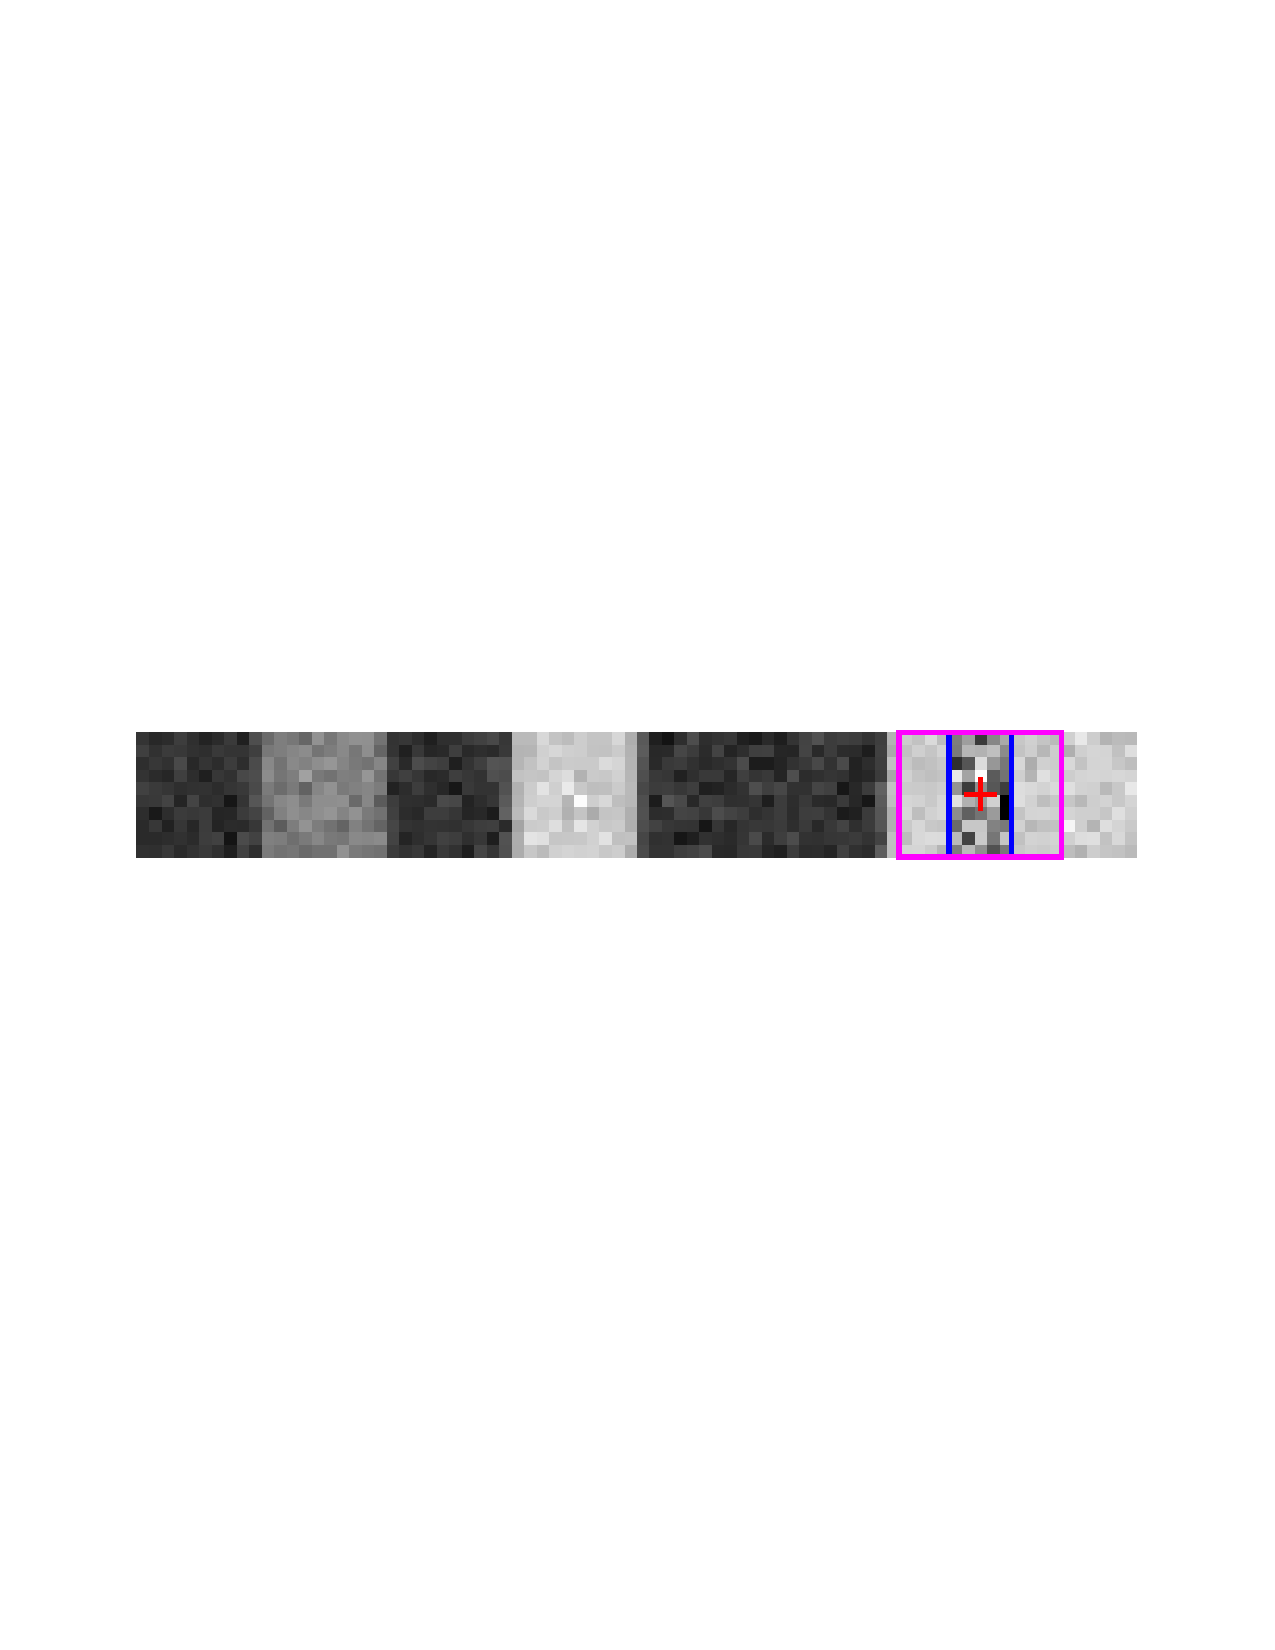
\includegraphics[width=\textwidth]{paper/latex/figures/high_resolution_success_imL_fine.png}
    \vspace{-15pt}
\end{subfigure}
\begin{subfigure}[t]{0.53\textwidth}
    \includegraphics[width=\textwidth]{paper/latex/figures/low_resolution_success_imL_fine.png}\\
    \vspace{-15pt}
\end{subfigure}
}

\makebox[\textwidth][c]{
\begin{subfigure}[t]{0.53\textwidth}
    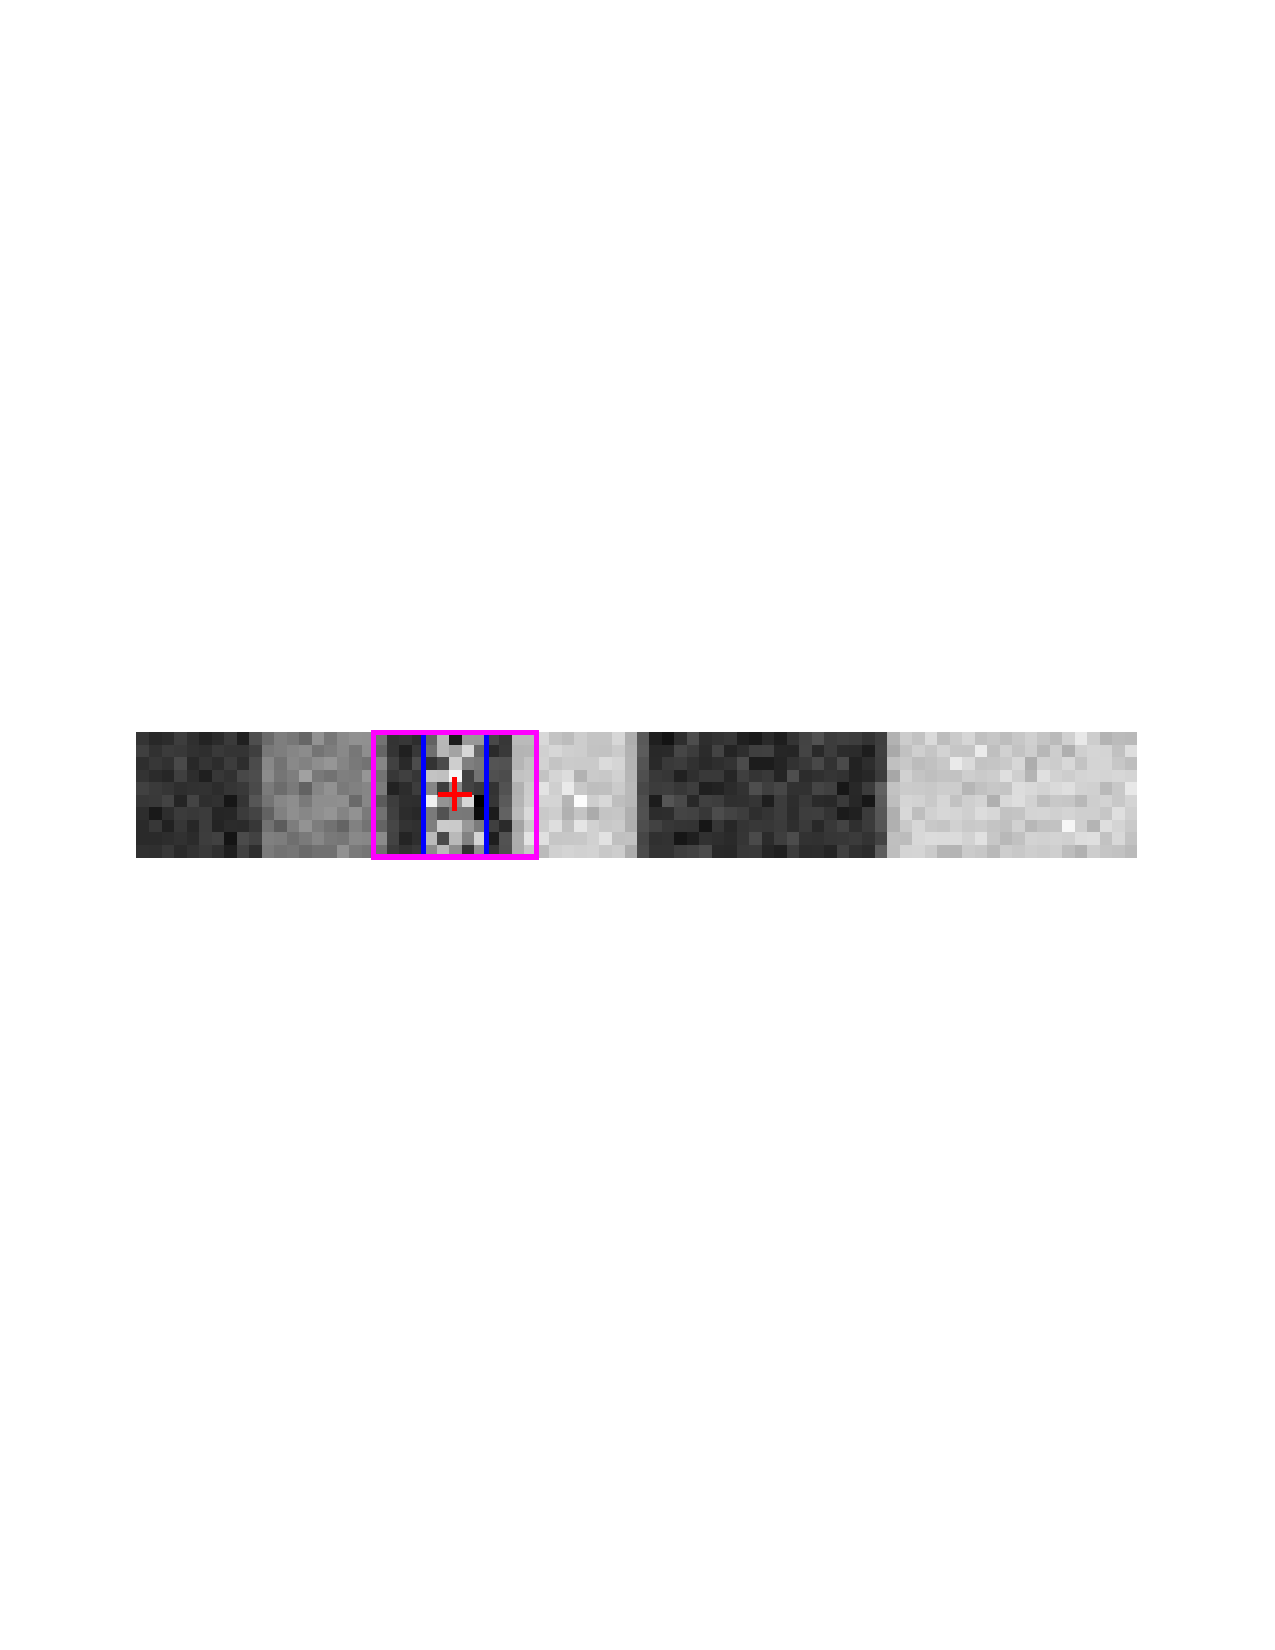
\includegraphics[width=\textwidth]{paper/latex/figures/high_resolution_success_imR_fine.png}
    \vspace{-15pt}
\end{subfigure}
\begin{subfigure}[t]{0.53\textwidth}
    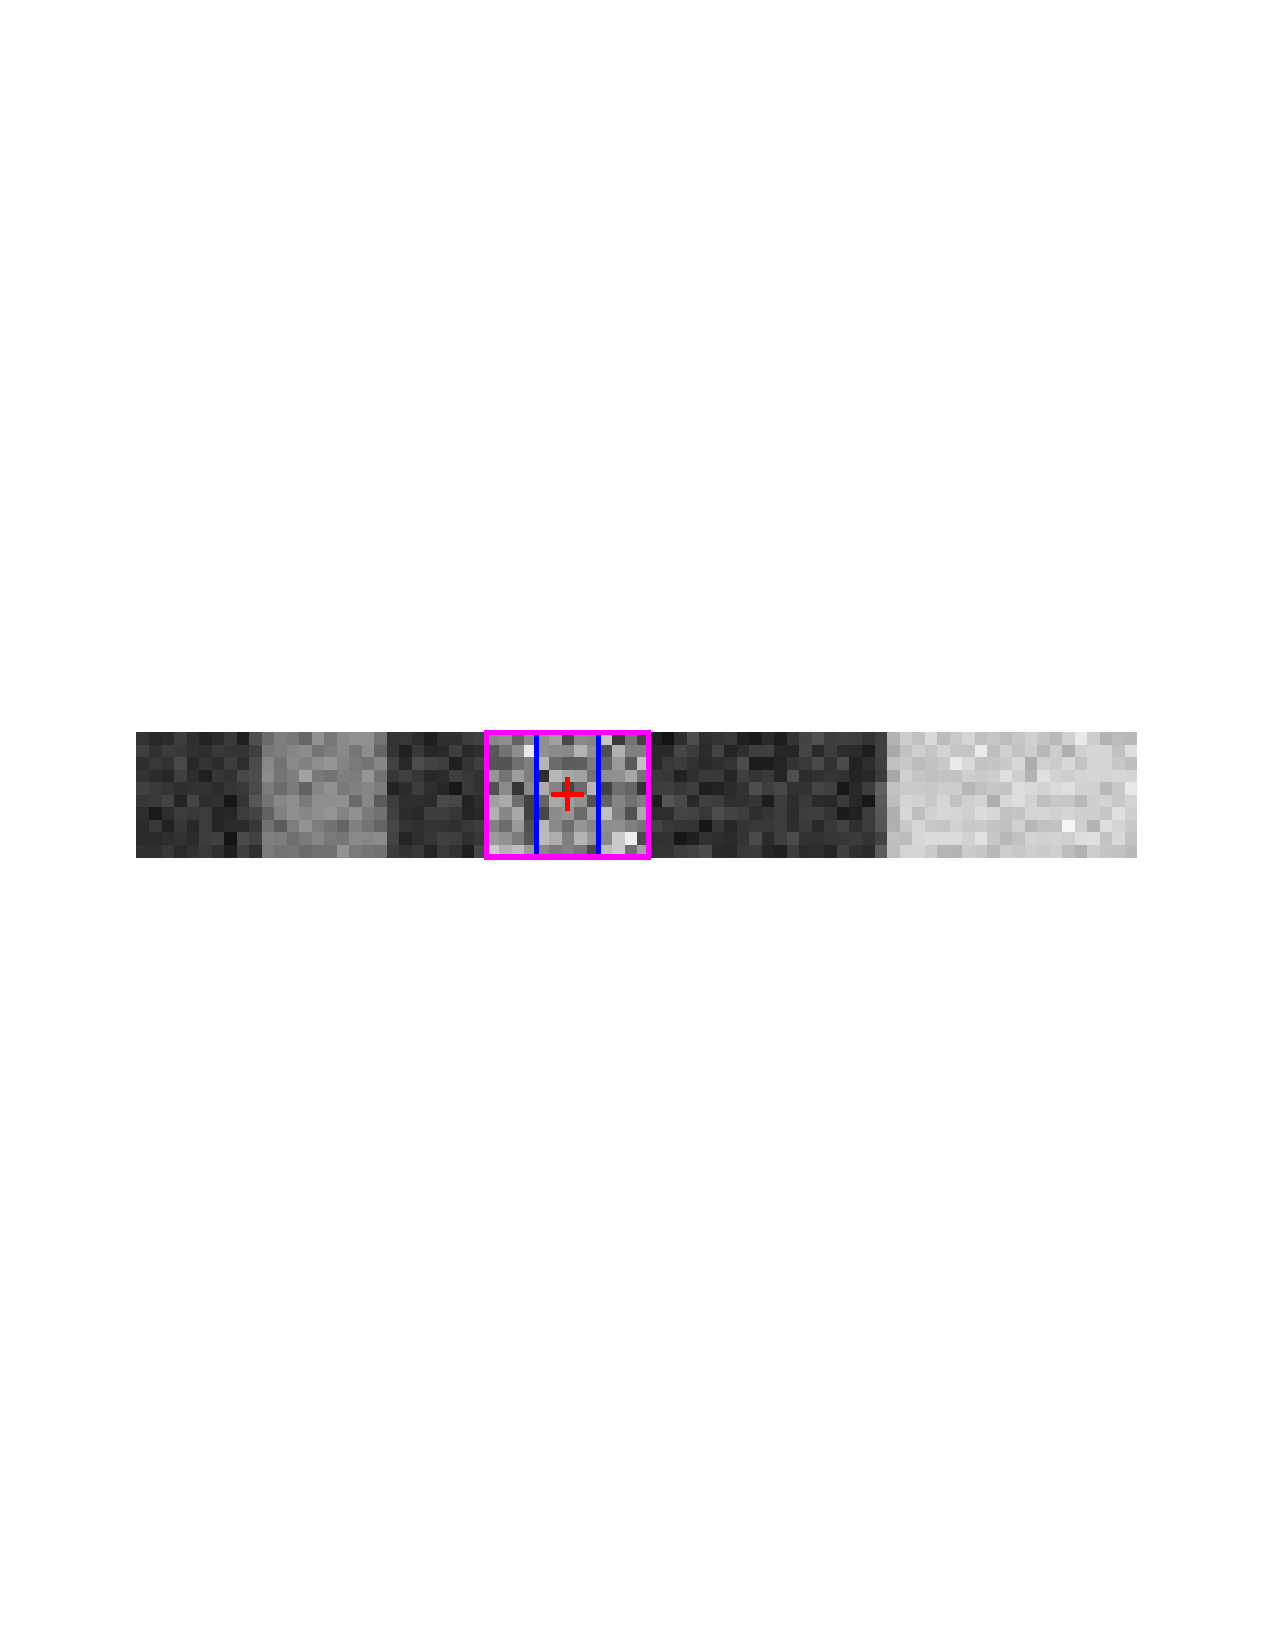
\includegraphics[width=\textwidth]{paper/latex/figures/low_resolution_success_imR_fine.png}\\
    \vspace{-15pt}
\end{subfigure}
}

\makebox[\textwidth][c]{
\begin{subfigure}[t]{0.53\textwidth}
    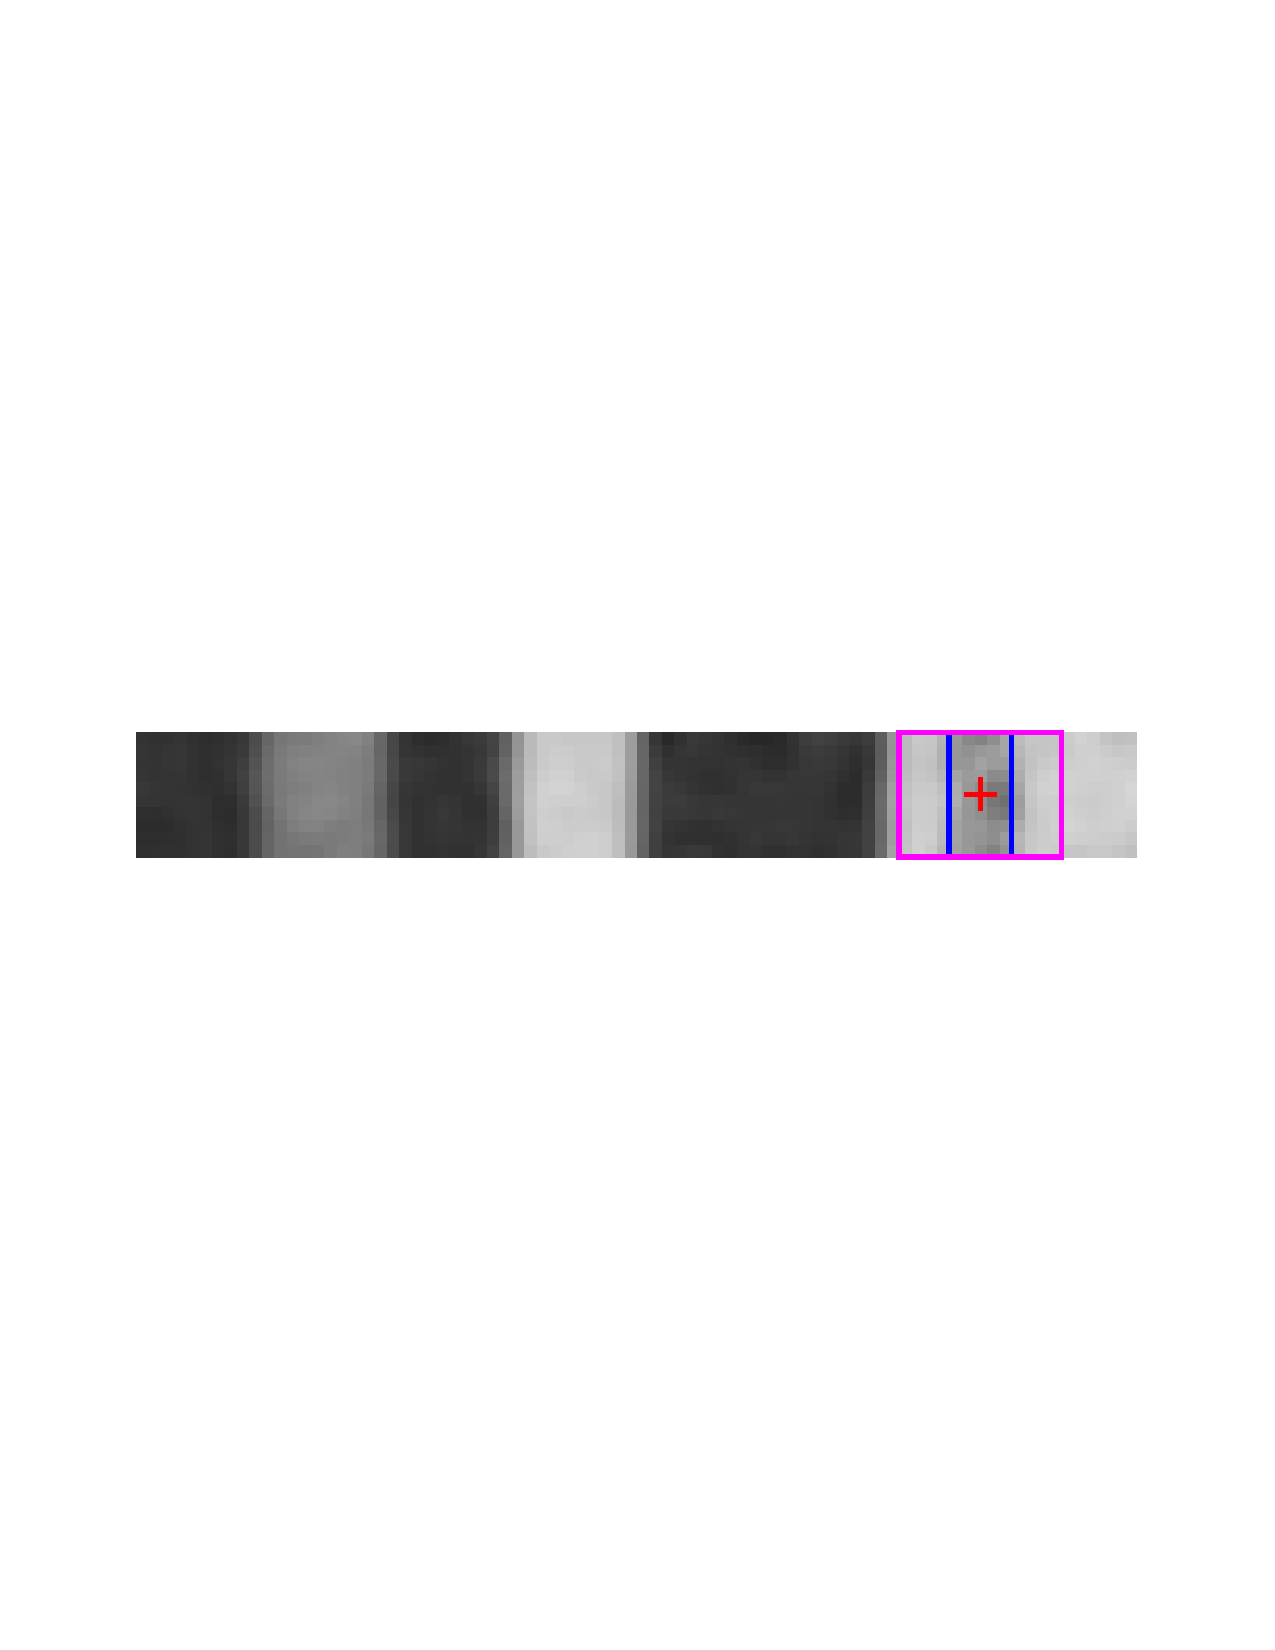
\includegraphics[width=\textwidth]{paper/latex/figures/high_resolution_success_imL_coarse.png}
    \vspace{-15pt}
\end{subfigure}
\begin{subfigure}[t]{0.53\textwidth}
    \includegraphics[width=\textwidth]{paper/latex/figures/low_resolution_success_imL_coarse.png}\\
    \vspace{-15pt}
\end{subfigure}
}

\makebox[\textwidth][c]{
\begin{subfigure}[t]{0.53\textwidth}
    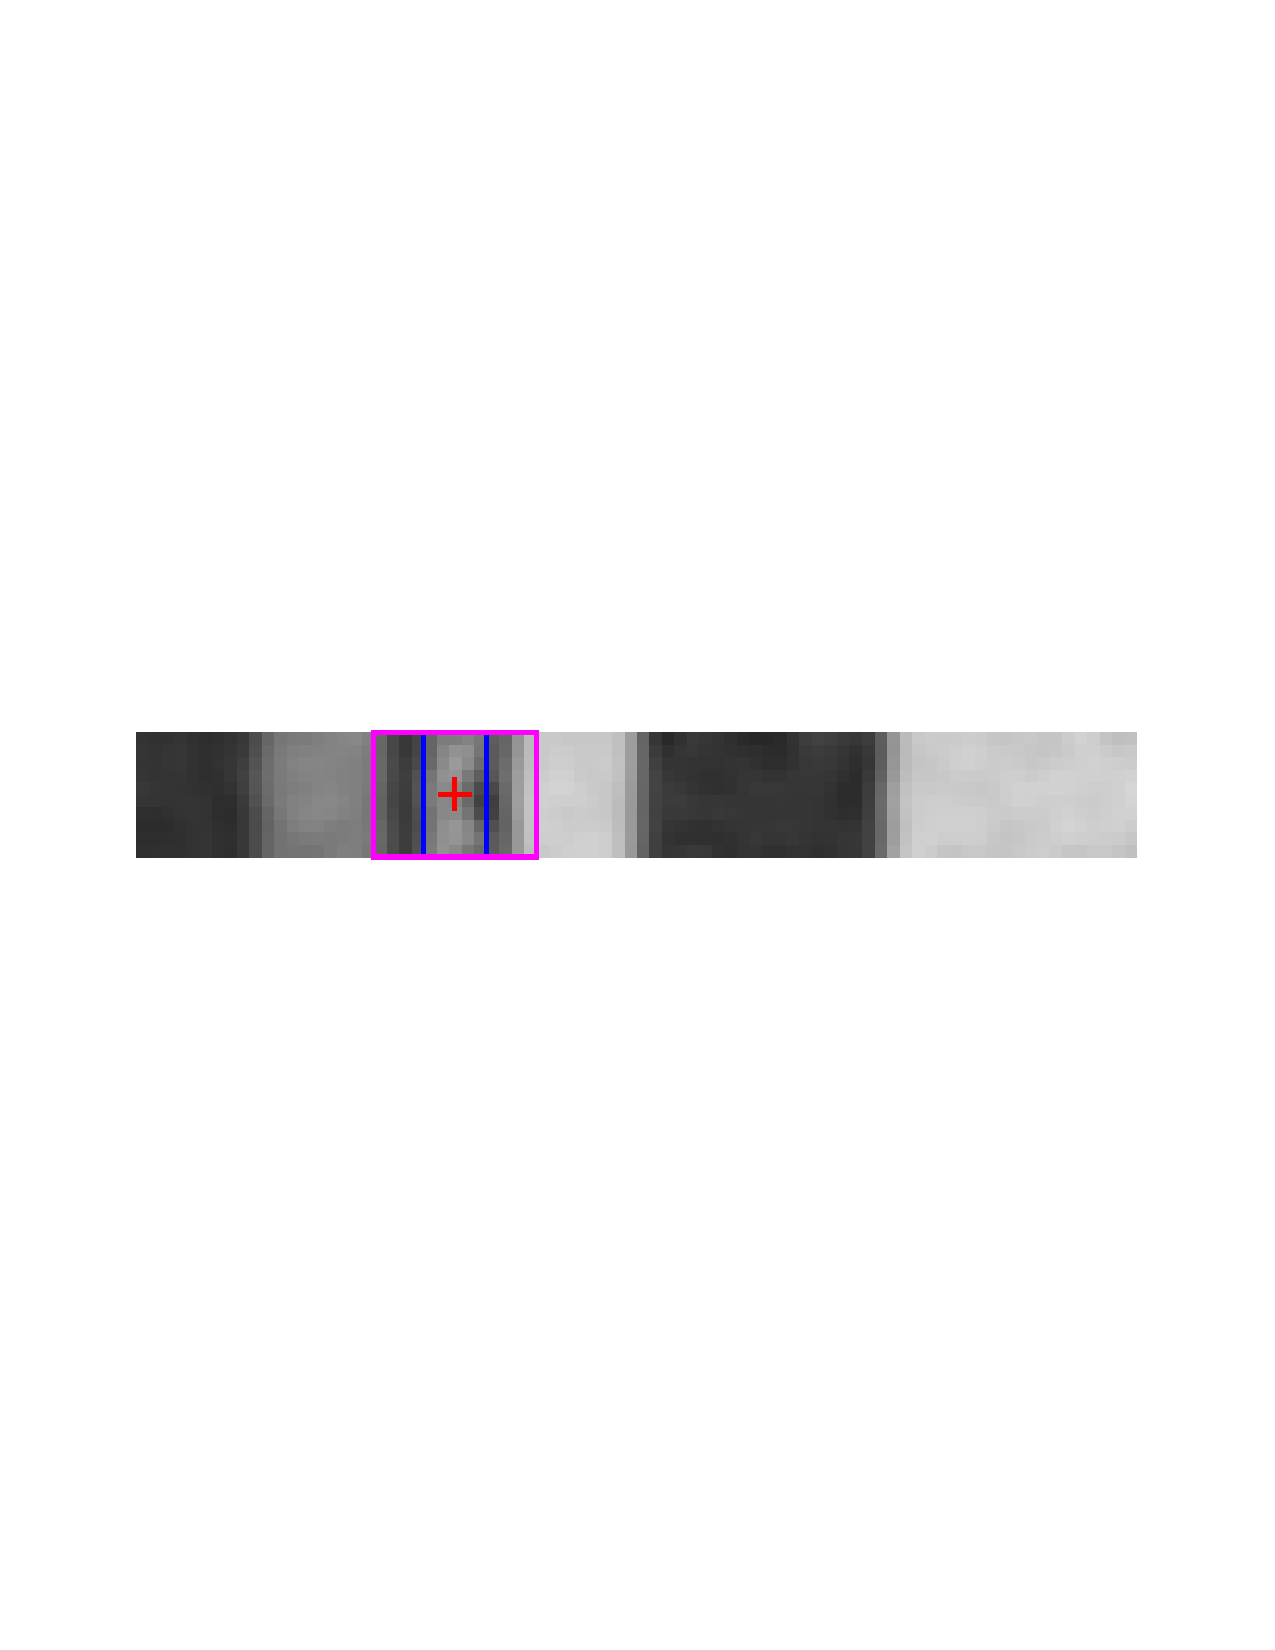
\includegraphics[width=\textwidth]{paper/latex/figures/high_resolution_success_imR_coarse.png}
    \vspace{-5pt}
\end{subfigure}
\begin{subfigure}[t]{0.53\textwidth}
    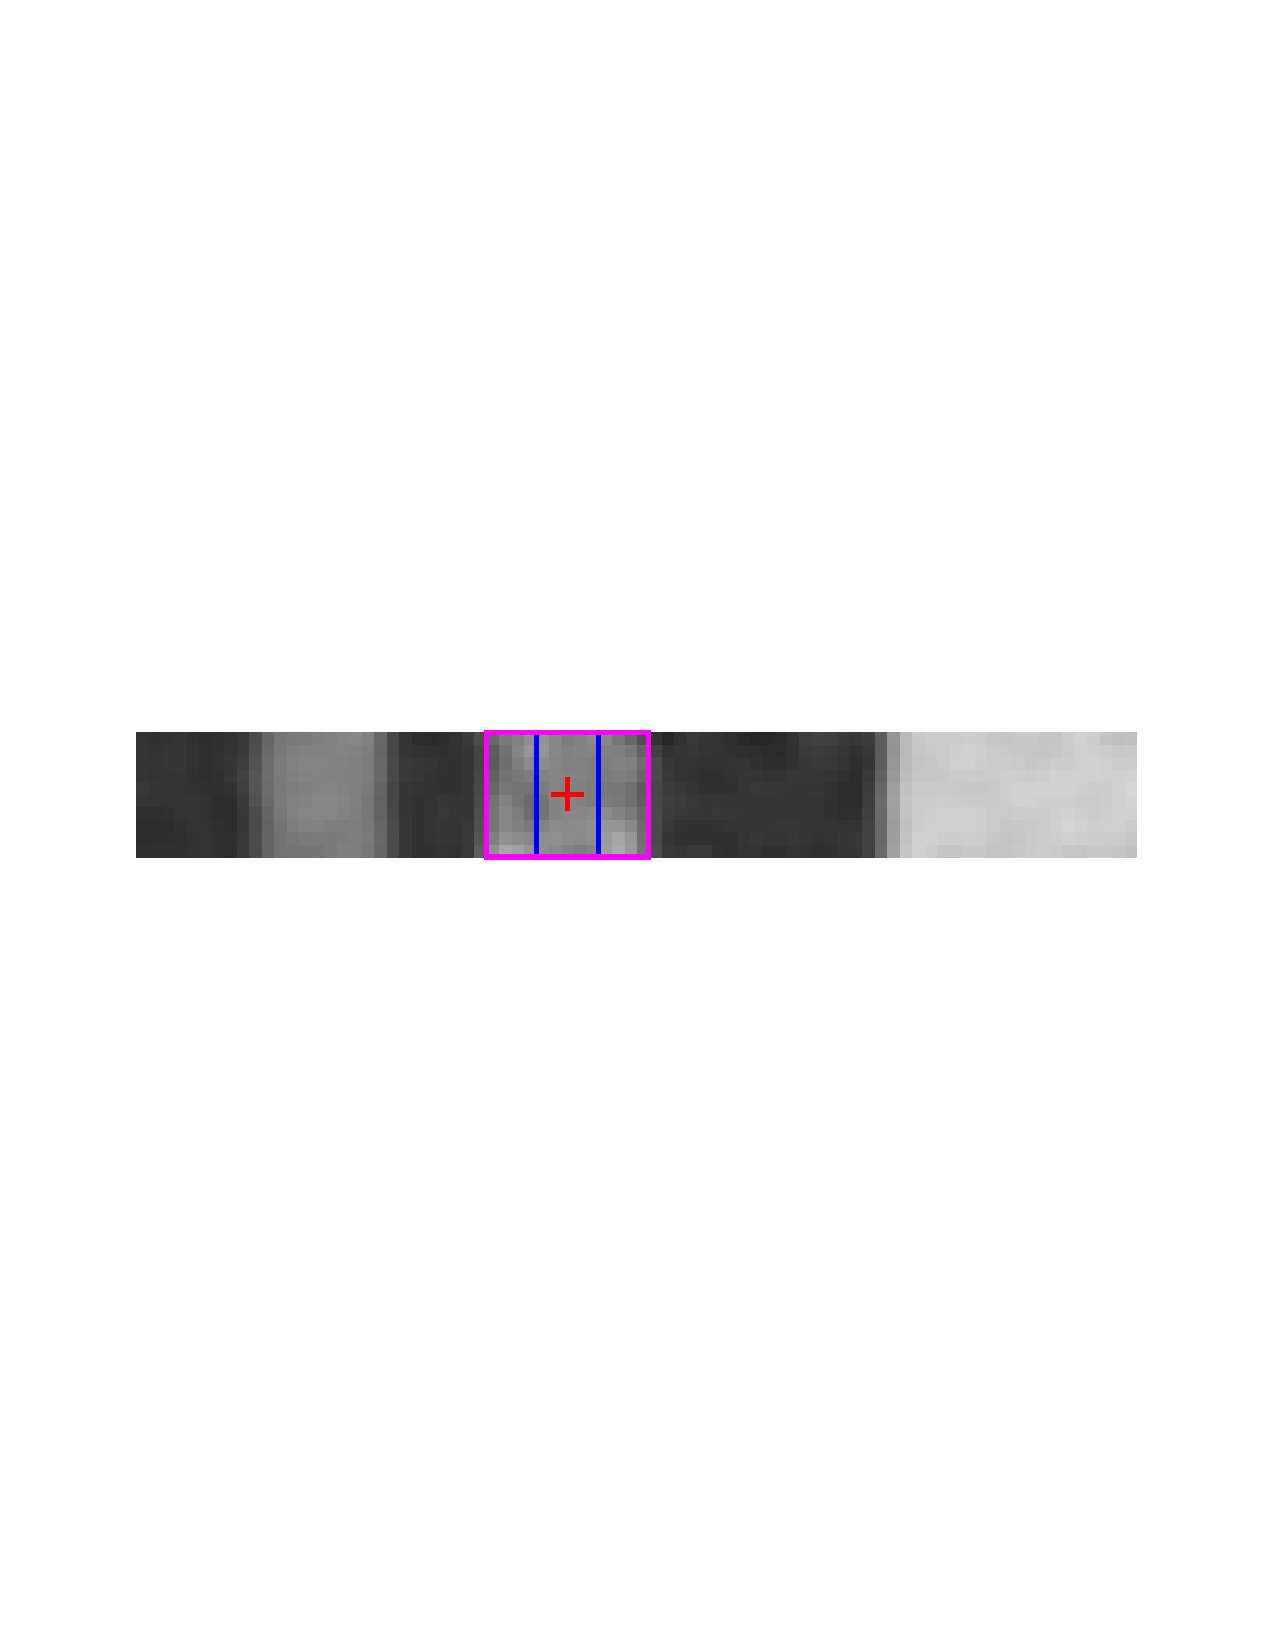
\includegraphics[width=\textwidth]{paper/latex/figures/low_resolution_success_imR_coarse.png}\\
    \vspace{-5pt}
\end{subfigure}
}

\makebox[\textwidth][c]{
\begin{subfigure}[t]{0.54\textwidth}
    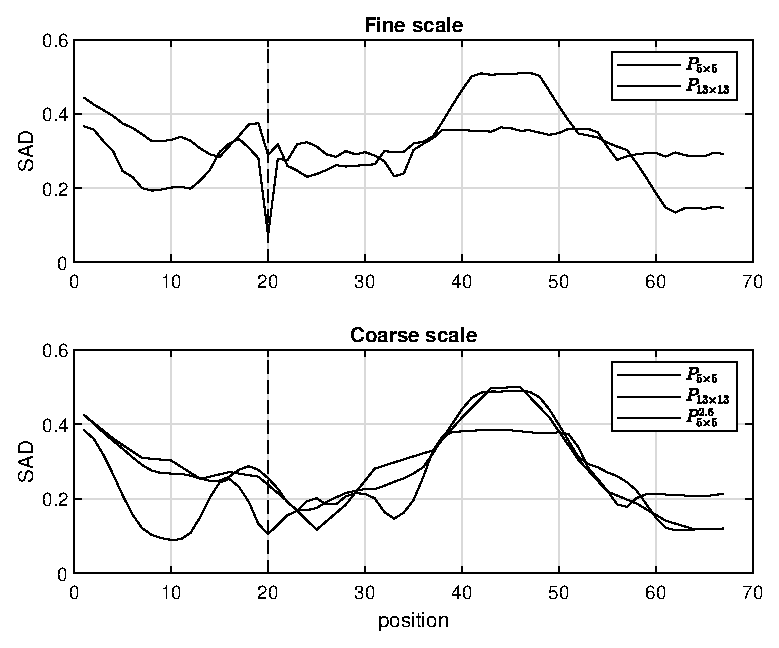
\includegraphics[width=\textwidth]{paper/latex/figures/high_resolution_success_graph.eps}
    \vspace{-10pt}
\end{subfigure}
\begin{subfigure}[t]{0.54\textwidth}
    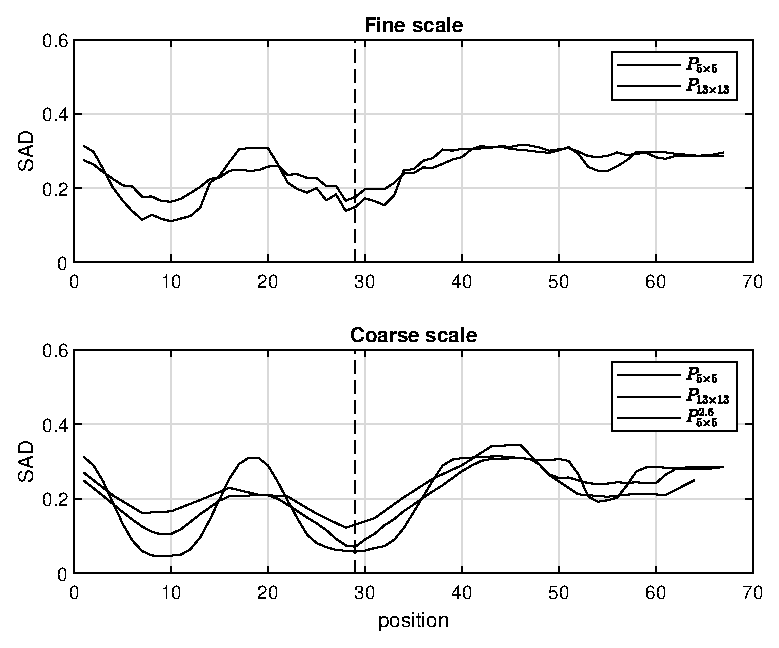
\includegraphics[width=\textwidth]{paper/latex/figures/low_resolution_success_graph.eps}\\
    \vspace{-10pt}
\end{subfigure}
}
\vspace{-15pt}
\caption{In this figure, we draw a simple artificial example to demonstrate the importance of multiscale patch comparison. In the left column, the fine scale image combined with a small patch size $P_{5 \times 5}$ leads to an accurate disparity curve, whereas in the right example, this happens through the coarse scale and the bigger patch $P_{13 \times 13}$. In the right example, we can observe, that we can approach the same disparity curve by applying a small patch size ($5 \times 5$) after downsampling the coarse scale image at a rate $\sfrac{13}{5}$. This example verifies that instead of keep changing the patch size, we can keep it fixed and apply it to a scale-space pyramid of the stereo pair.}
\label{fig:multiscale_importance_2D}  
\vspace{-3pt}      
\end{figure*}
%%%%%%%%%%%%%%%%%%%%%%%%%%%%%%%%%%%%%%%%%%%%%%%%%%%%%%%%%%%%%%%%
%%%%%%%%%%%%%%%%%%%%%%%%%%%%%%%%%%%%%%%%%%%%%%%%%%%%%%%%%%%%%%%%

\subsection{Single-scale prediction}

In this section, we describe a simple cnn architecture for predicting disparity, respecting the stereo vision geometry particularities. In general, end-to-end techniques attempt to learn a direct mapping $\hat{Y} = f(X^L, X^R)$, for $\hat{Y}$ to be as close as possible to the ground truth disparity image $Y$. Taking advantage of basic stereo vision restrictions, this rather generic problem statement, can be divided into three subproblems:

\begin{itemize}
    \item Learning a method $f_1$ (2D cnn) for mapping every point $p$ of raw images $X^L, X^R$ to a descriptor $\vec{k} \in R^K$, creating descriptor images $X^L_{desc}, X^R_{desc}$. This feature space representation enables incorporating information from local context for creating robust descriptors, on which forthcoming similarity comparisons will be based upon.
    
    \item Design a method $g_1$ for forming the comparison volume $C$. This step is usually hand-crafted and does not contain a learnable method. In our proposed method, instead of just concatenating the descriptors of compared points, we design a more concise method $g_1$, avoiding the redundancy introduced by simple concatenation. We explain in depth our method at section \ref{sec:comparison_volume}.
    
    \item Learning a method $f_2$ (3d cnn) for predicting the disparity image $\hat{D}$. We follow the methodology proposed in \cite{Kendall2017End-to-EndRegression}, where $f_2$ learns a mapping from the comparison volume $C$ to the similarity volume $S$ through a $3D$ convolutional network. The similarity volume stores a probability $p \in [0,1] $ for each correspondence $S[d,x,y] = p$. Afterwards, a $g_2=softargmax$ operator applied along $d$ dimension, is used for obtaining the final disparity prediction.
\end{itemize}

Combining the aforementioned parts, we create the following cnn architecture which can be trained end-to-end:

\begin{equation} \label{eq:single_scale_architecture}
    \hat{Y} = f(X^L, X^R) = g_2 ( f_2 ( g_1 ( f_1(X^L), f_1(X^R) ) ) )
\end{equation}

Equation \ref{eq:single_scale_architecture} implements the prediction mechanism at the highest resolution of the input images. Instead, we could apply the same procedure at any coarser scale by intervening two simple layers:

\begin{itemize}
    \item A downscaling layer $L_1^t: \mathbb{R}^{H \times W} \rightarrow \mathbb{R}^{\sfrac{H}{t} \times \sfrac{W}{t}}$, where $t$ represents the downsampling factor. $L_1^t$ applies sequentially a gaussian kernel $k(x, y, \sigma) = \frac{1}{2\pi\sigma^2} \cdot e^{\sfrac{-(x^2 + y^2)}{2\sigma^2}}$, where $\sigma = \sfrac{t}{3}$ and a bilinear downsampling layer.
    
    \item A trilinear upsampling mechanism $L_2^t: \mathbb{R}^{D \times H \times W} \rightarrow \mathbb{R}^{tD \times tH \times tW}$, where $t$ represents the upsampling factor.
\end{itemize}

Hence, intervening those two simple layers we enforce the procedure \ref{eq:single_scale_architecture} to take place at specific scale $t$:

\begin{equation} \label{eq:single_scale_archtecture_at_sigma}
    \hat{Y}^t = f^t(X^L, X^R) = g_2( L_2^t (f_2 ( g_1 ( f_1(L_1^t(X^L)), f_1(L_1^t(X^R)) ) ) ) )
\end{equation}


\subsection{Multi-scale fusion}

Exploiting information from different scales is the crucial task of our proposed method. As mentioned, there are regions of the image where coarser scales provide more accurate estimations and vice-versa. Let's define a coarse scale comparison volume $C^{t_2}$ and a corresponding fine scale $C^{t_1}$. Our target is to learn a method that can locate the trustable information from the different scales and incorporate it to produce a mixed scale volume $C^{t_2, t_1}$. Our intuition for designing this learning structure, follows the following schema; If both scales vote for the same disparity estimation, this estimation must be strengthened. If a conflict is found, the network should decide which prediction to follow (fine or coarse) by appraising the robustness of each disparity curve. Finally, if neither prediction is robust this info must be imprinted to the produced tensor.

The finer scale volume $C^{t_1}$ passes through the $3D$ cnn $f_3: \mathbb{R}^{D \times H \times W \times K_1} \rightarrow  \mathbb{R}^{D \times H \times W \times K_2}$, which is responsible for preparing it for concatenation. The coarser scale volume $C_2$ is upsampled through a trillinear upsampling layer $L_2^{\sfrac{t_2}{t_1}}$ and it is concatenated with $C^{t_1}$. Finally, another $3D$ cnn $f_4: \mathbb{R}^{D \times H \times W \times 2K_2} \rightarrow  \mathbb{R}^{D \times H \times W \times K_2}$ gets the concatenated  projects it to initial input space. Equation \ref{eq:two_scale_fusion} represents the basic construction block of the proposed method and Algorithm \ref{alg:multi_scale_fusion} the whole repetitive procedure for combining information for all scales.

\begin{equation} \label{eq:two_scale_fusion}
C^{ \{ t_n, ..., t_{i+1}, t_{i} \} } = f_4(L_2^{\sfrac{t_{i+1}}{t_i} }(C^{ \{ t_n, ..., t_{i+1} \} }), f_3(C^{t_i}) )
\end{equation}


\begin{algorithm}
\caption{Multi-scale fusion}\label{alg:multi_scale_fusion}
\begin{algorithmic}[1]
\Procedure{multi scale fusion}{$ C^{t_n}, \cdot \cdot \cdot, C^{t_0} $}
\State $C_1 \gets f_3(C^{t_n})$ \Comment{Init coarse scale volume}
\For { \texttt{i=n-1;-1;0} }
\State $C_1 \gets L_2^{\sfrac{ t_{i+1} }{ t_i } }(C_1)$ \Comment{3D Upsampling}
\State $C_2 \gets f_3(C^{t_i})$ \Comment{Prepare finer scale volume}
\State $C_1 \gets f_4(C_1, C_2)$ \Comment{Concatenate and project to input space}
\EndFor
\State \Return $C_1$
\EndProcedure
\end{algorithmic}
\end{algorithm}


\subsection{Comparison volume} \label{sec:comparison_volume}

The comparison volume is used as a helping step for zipping comparison information into a 3D tensor $\mathbb{R}^{D \times H \times W} \rightarrow \mathbb{R}^K$. Normally, the comparison volume is formed by simply concatenating the descriptors compared points $C[d, x, y]  = X^L_{desc}(x,y) \oplus  X^R_{desc}(x-d,y)$. Although this method retains all descriptors intact, it introduces significant redundancy; rearranges $H \times W \times K$ unique values into an object of $D \times H \times Y \times 2K$ total values. For keeping the computational complexity low, we compute similarity measure between each corresponding value of the descriptors under comparison. Afterwards, we concatenate the initial left image $X^L$ along axis $d$ for incorporating the local context information. We symbolize the whole procedure as $g_1$.

\begin{equation}
\begin{gathered} \label{eq:comparison_volume}
    g: \mathbb{R}^2 \rightarrow \mathbb{R}: g(a_1, a_2) = \frac{|a_1 + a_2|}{2} \cdot e^{-|a_1 - a_2|} \\
    C_1^t[d, x, y, i] = g( X^{L, t}_{desc}[x,y,i], X^{R, t}_{desc}[x-d,y, i]) \\
    C^t = X^{L, t} \oplus C_1^t
\end{gathered}
\end{equation}

\subsection{Cnn architectures}

In this section we present the specific cnn architectures used as the learnable parts of our model (i.e. functions $f_1, f_2, f_3, f_4$).

\begin{figure}
    \centering
    \includegraphics[width = \textwidth]{paper/latex/figures/cnn_architecture.png}
    \caption{Scale fusion network overview. Its main constructive blocks are the horizontal pipelines (green colour) representing end-to-end predictions at specific scale $\sigma$ and the vertical pipelines (grey colour) representing the pair-scales fusion at similarity matrix level. The red-coloured blocks are the learned parts of our architecture, while the yellow coloured ones are hand-crafted layers.}
    \label{fig:cnn_architecture}
\end{figure}

\begin{table}[]
    \centering
    \begin{tabular}{ l|c|c|c }
    Name & Symbol & Set & Formula \rule{0pt}{2ex}\\
    
    \hline
    \multicolumn{4}{c}{ \textbf{Definitions} } \rule{0pt}{2.4ex}\\
    \hline
    
    Raw image & $X^L, X^R$ & $\mathbb{R}^{H \times W \times 3}$ & -  \rule{0pt}{2.5ex} \\
    
    Ground truth & $Y$ & $\mathbb{R}^{H \times W}$ & - \rule{0pt}{2.5ex} \\
    
    \hline
    \multicolumn{4}{c}{ \textbf{Single-Scale 2D Processing} } \rule{0pt}{2.4ex}\\
    \hline
    
    Downsampled image & $X^{L,t}, X^{R, t}$ & $\mathbb{R}^{\sfrac{H}{t} \times \sfrac{W}{t} \times 3}$ & $L_1^t(X^L), L_1^t(X^R)$  \rule{0pt}{3ex} \\
    
    Descriptor image & $X^{L,t}_{desc}, X^{R, t}_{desc}$ & $\mathbb{R}^{\sfrac{H}{t} \times \sfrac{W}{t} \times K}$ & $f_1(X^{L,t}), f_1(X^{R, t})$  \rule{0pt}{3.5ex} \rule[-1.3ex]{0pt}{0pt}\\
    
    \hline
    \multicolumn{4}{c}{ \textbf{Single-Scale 3D Processing} } \rule{0pt}{2.4ex}\\
    \hline
    
    Comparison volume & $C^{t}$ & $ \mathbb{R}^{ \sfrac{D}{t} \times \sfrac{H}{t} \times \sfrac{W}{t} \times K' }  $  & $g_1(X^{L,t}_{desc}, X^{R, t}_{desc}, X^{L,t})$ \rule{0pt}{3ex} \\
    
    Similarity volume & $S^{t}$ & $ \mathbb{R}^{ \sfrac{D}{t} \times \sfrac{H}{t} \times \sfrac{W}{t}} $  & $f_2(C^{t})$ \rule{0pt}{3.5ex} \\
    
    Prediction image & $\hat{Y}^{t}$ & $\mathbb{R}^{H \times W}$ & $ g_2(t_2^{t}(S^{t}))$ \rule{0pt}{3.5ex} \\
    
    \hline
    \multicolumn{4}{c}{ \textbf{Multi-Scale 3D Processing} } \rule{0pt}{2.4ex} \\
    \hline
    
    Comparison volume & $C^{ \{ t_n, ... , t_0 \} }$ & $ \mathbb{R}^{ \sfrac{D}{t_0} \times \sfrac{H}{t_0} \times \sfrac{W}{t_0} \times K' }  $  & $\text{MultiScaleFusion}(C^{t_n}, ..., C^{t_0})$ \rule{0pt}{3ex} \\
    
    Similarity volume & $S^{ \{ t_n, ... , t_0 \} }$ & $ \mathbb{R}^{ \sfrac{D}{t_0} \times \sfrac{H}{t_0} \times \sfrac{W}{t_0}} $  & $f_2(C^{ \{ t_n, ... , t_0 \} })$ \rule{0pt}{3.5ex} \\
    
    Prediction image & $\hat{Y}^{ \{ t_n, ... , t_0 \} }$ & $\mathbb{R}^{ H \times W}$ & $g_2 (L_2^{t_0}(S^{ \{ t_n, ... , t_0 \} }))$ \rule{0pt}{3.5ex} \\
    \hline
    \end{tabular}
    \caption{Description of all tensors involved in the proposed method}
    \label{tab:entity_description}
\end{table}

\subsection{Weight sharing}

Our method is based on some constructive blocks that can be combined in any arbitrary combination of scales. This specification provides some scalability to the network which can thought as a tweaking capability between conflicting characteristics. If one targets for accuracy, he can combine many different scales of processing. On the other hand, if one targets for faster processing times, has less computational resources or does not care for complex details in the disparity prediction, he may choose less and coarser points in the scale space.

In the experimental part, we show that repeating the same constructive blocks, which can be thought as weight sharing between some layers, doesn't decrease network's expressiveness.

%%%%%%%%%%%%%%%%%%%%%%%%%%%%%%%%%%%%%%%%%%%%%%%%%%%%%%%%%%%%%%%%%
\section{Experimental evaluation}

In this section we provide some quantitative and qualitative results of our proposed methods on the large synthetic SceneFlow dataset. In section \ref{sec:4_1}, we show  how the multi-scale fusion algorithm adopts progressively the coarse to fine information. In section \ref{sec:4_2}, we compare the proposed network to the state-of-the-art methods, at SceneFlow dataset. In section ..., we compare the proposed network to some more generic architecture, showing that enforcing the multi-scale process leads to better results even with less trainable parameters. In section ..., we compare the proposed network to the ones following the same architecture without weight sharing.

\subsection{Multi-Scale fusion analysis} \label{sec:4_1}

In figure \ref{fig:multiscale_importance}, we show how our 3D cnn network has learned incorporating and progressively adopting fine scale predictions. We choose two different type image points, one appropriate for fine scale prediction on fine and the other on coarse scale. We ascertain that multi-scale fusion algorithm, counts on the correct scale in each case, without inserting error from other scales. In figure \ref{fig:EMAPs}, we demonstrate predictions of the same input stereo pair at single and multi-scale mode.  

%%%%%%%%%%%%%%%%%%%%%%%%%%%%%%%%%%%%%%%%%%%%%%%%%%%%%%%%%%%%%%%%
%%%%%%%%%%%%%%%%% Multiscale 3d importance %%%%%%%%%%%%%%%%%%%%%
\begin{figure*}[t]
\centering
\makebox[\textwidth][c]{
    \begin{subfigure}[b]{0.5\textwidth}
        \includegraphics[width=\textwidth]{paper/latex/figures/multiscale_importance_image_patches.pdf}\\
        \vspace{-15pt}                
    \end{subfigure} 
}
\centering
\makebox[\textwidth][c]{
    \begin{subfigure}[b]{1.15\textwidth}
        \includegraphics[width=\textwidth]{paper/latex/figures/multiscale_importance_graph_high_resolution.pdf}\\
        \vspace{-15pt}                
    \end{subfigure} 
}
\centering
\makebox[\textwidth][c]{
    \begin{subfigure}[b]{1.15\textwidth}
        \includegraphics[width=\textwidth]{paper/latex/figures/multiscale_importance_graph_low_resolution.pdf}\\
        \vspace{-15pt}                
        \caption{In this figure, we compare two regions of the same image that require processing on different scale. The centre point of the yellow rectangle is a small object on the foreground with many features (i.e. handle of a knife), whilst the orange one represents a background area inside a repetitive pattern. The first column of graphs represents the Multi-Scale similarity volumes $S^{\{ \sigma_0, ..., \sigma_n \} }$ The graphs prove that, as we expected, disparity estimation is accurate on higher scale for the yellow rectangle and on t As expected,  }
    \end{subfigure} 
}
\vspace{-15pt}
\caption{TEXT}
\label{fig:multiscale_importance}  
\vspace{-3pt}      
\end{figure*}
%%%%%%%%%%%%%%%%%%%%%%%%%%%%%%%%%%%%%%%%%%%%%%%%%%%%%%%%%%%%%%%%
%%%%%%%%%%%%%%%%%%%%%%%%%%%%%%%%%%%%%%%%%%%%%%%%%%%%%%%%%%%%%%%%

%%%%%%%%%%%%%%%%%%%%%%%%%%%%%%%%%%%%%%%%%%%%%%%%%%%%%%%%%%%%%%%%
%%%%%%%%%%%%%%%%%%%%%%%%%%%%%%%%%%%%%%%%%%%%%%%%%%%%%%%%%%%%%%%%
\begin{figure*}[t]
\centering
\makebox[\textwidth][c]{
    \begin{subfigure}[b]{0.28\textwidth}
        \includegraphics[width=\textwidth]{paper/latex/figures/imL_0.png}\\
        \vspace{-15pt}                
        \caption{$X^{L,1}$}
    \end{subfigure} 
    \hspace{0.001cm} 
    \begin{subfigure}[b]{0.28\textwidth}
        \includegraphics[width=\textwidth]{paper/latex/figures/imL_1.png}\\
        \vspace{-15pt}      
        \caption{$X^{L,2}$}
    \end{subfigure} 
    \hspace{0.001cm} 
    \begin{subfigure}[b]{0.28\textwidth}
        \includegraphics[width=\textwidth]{paper/latex/figures/imL_2.png}\\
        \vspace{-15pt}                      
        \caption{$X^{L,4}$}
    \end{subfigure} 
    \hspace{0.001cm} 
    \begin{subfigure}[b]{0.28\textwidth}
        \includegraphics[width=\textwidth]{paper/latex/figures/imL_3.png}\\
        \vspace{-15pt}     
        \caption{$X^{L,8}$}
    \end{subfigure}         
}
\centering
\makebox[\textwidth][c]{
    \begin{subfigure}[b]{0.28\textwidth}
        \includegraphics[width=\textwidth]{paper/latex/figures/pred_comb_0.png}\\
        \vspace{-15pt}                
        \caption{$\hat{D}_{comb}^{L,1}$}
    \end{subfigure} 
    \hspace{0.001cm} 
    \begin{subfigure}[b]{0.28\textwidth}
        \includegraphics[width=\textwidth]{paper/latex/figures/pred_comb_1.png}\\
        \vspace{-15pt}      
        \caption{$\hat{D}_{comb}^{L,2}$}
    \end{subfigure} 
    \hspace{0.001cm} 
    \begin{subfigure}[b]{0.28\textwidth}
        \includegraphics[width=\textwidth]{paper/latex/figures/pred_comb_2.png}\\
        \vspace{-15pt}                      
        \caption{$\hat{D}_{comb}^{L,4}$}
    \end{subfigure} 
    \hspace{0.001cm} 
    \begin{subfigure}[b]{0.28\textwidth}
        \includegraphics[width=\textwidth]{paper/latex/figures/pred_comb_3.png}\\
        \vspace{-15pt}     
        \caption{$\hat{D}_{comb}^{L,8}$}
    \end{subfigure}         
}
\centering
\makebox[\textwidth][c]{
    \begin{subfigure}[b]{0.28\textwidth}
        \includegraphics[width=\textwidth]{paper/latex/figures/pred_comb_0_err.png}\\
        \vspace{-15pt}                
        \caption{$E_{comb}^{L,1}$}
    \end{subfigure} 
    \hspace{0.001cm} 
    \begin{subfigure}[b]{0.28\textwidth}
        \includegraphics[width=\textwidth]{paper/latex/figures/pred_comb_1_err.png}\\
        \vspace{-15pt}      
        \caption{$E_{comb}^{L,2}$}
    \end{subfigure} 
    \hspace{0.001cm} 
    \begin{subfigure}[b]{0.28\textwidth}
        \includegraphics[width=\textwidth]{paper/latex/figures/pred_comb_2_err.png}\\
        \vspace{-15pt}                      
        \caption{$E_{comb}^{L,4}$}
    \end{subfigure} 
    \hspace{0.001cm} 
    \begin{subfigure}[b]{0.28\textwidth}
        \includegraphics[width=\textwidth]{paper/latex/figures/pred_comb_3_err.png}\\
        \vspace{-15pt}     
        \caption{$E_{comb}^{L,8}$}
    \end{subfigure}         
}
\centering
\makebox[\textwidth][c]{
    \begin{subfigure}[b]{0.28\textwidth}
        \includegraphics[width=\textwidth]{paper/latex/figures/pred_0.png}\\
        \vspace{-15pt}                
        \caption{$\hat{D}^{L,1}$}
    \end{subfigure} 
    \hspace{0.001cm} 
    \begin{subfigure}[b]{0.28\textwidth}
        \includegraphics[width=\textwidth]{paper/latex/figures/pred_1.png}\\
        \vspace{-15pt}      
        \caption{$\hat{D}^{L,2}$}
    \end{subfigure} 
    \hspace{0.001cm} 
    \begin{subfigure}[b]{0.28\textwidth}
        \includegraphics[width=\textwidth]{paper/latex/figures/pred_2.png}\\
        \vspace{-15pt}                      
        \caption{$\hat{D}^{L,4}$}
    \end{subfigure} 
    \hspace{0.001cm} 
    \begin{subfigure}[b]{0.28\textwidth}
        \includegraphics[width=\textwidth]{paper/latex/figures/pred_3.png}\\
        \vspace{-15pt}     
        \caption{$\hat{D}^{L,8}$}
    \end{subfigure}         
}
\centering
\makebox[\textwidth][c]{
    \begin{subfigure}[b]{0.28\textwidth}
        \includegraphics[width=\textwidth]{paper/latex/figures/pred_0_err.png}\\
        \vspace{-15pt}                
        \caption{$E^{L,1}$}
    \end{subfigure} 
    \hspace{0.001cm} 
    \begin{subfigure}[b]{0.28\textwidth}
        \includegraphics[width=\textwidth]{paper/latex/figures/pred_1_err.png}\\
        \vspace{-15pt}      
        \caption{$E^{L,2}$}
    \end{subfigure} 
    \hspace{0.001cm} 
    \begin{subfigure}[b]{0.28\textwidth}
        \includegraphics[width=\textwidth]{paper/latex/figures/pred_2_err.png}\\
        \vspace{-15pt}                      
        \caption{$E^{L,4}$}
    \end{subfigure} 
    \hspace{0.001cm} 
    \begin{subfigure}[b]{0.28\textwidth}
        \includegraphics[width=\textwidth]{paper/latex/figures/pred_3_err.png}\\
        \vspace{-15pt}     
        \caption{$E^{L,8}$}
    \end{subfigure}         
}
\vspace{-15pt}
\caption{TEXT}
\label{fig:EMAPs}  
\vspace{-3pt}      
\end{figure*}
%%%%%%%%%%%%%%%%%%%%%%%%%%%%%%%%%%%%%%%%%%%%%%%%%%%%%%%%%%%%%%%%

\subsection{SceneFlow benchmark} \label{sec:4_2}

In this section, we evaluate our network on the SceneFlow dataset. The evaluation process is undertaken at three separate parts, each one benchmarking a different perspective.

Firstly, we would like to check the benefit of enforcing explicitly the multiscale processing, instead of implementing a generic cnn architecture. For this purpose, we design 4 cnn architectures, following the designing principles of \ref{eq:single_scale_architecture}, changing only the specific layers that constitute $f_1$ and $f_2$. Specifically, the "OneRes" network's $f_1$ and $f_2$ consist of a pile of 2d and 3d residual blocks correspondingly. In "MRes2d", $f_1$ average pooling along with 2d upsampling layers have been added between 2d residual blocks, creating an stacked hourglass (encoding-decoding) architecture. In "MRes3d", the equivalent procedure at the 3d processing level, forms $f_2$. Finally, at "MRes2d3d", both $f_1$ and $f_2$ follow the encoder-decoder architecture. We implemented such models, since encoder-decoder architecture is a basic strategy that enables the network to adopt multiscale capabilities internally, through the training procedure. At table \ref{tab:results} and at graph \ref{fig:mae_SFNvsGenericNets} we observe that enforcing multiscale analysis leads to better accuracy, even with much less parameters.

Secondly, we question whether using the same constructive blocks $f_1$, $f_2$, $f_3$, $f_4$ repetitively between different scales lead to better results that leaving all model weights free along training. We must notice here that freeing the weights cancels the networks scalability, since the processing scales must be predefined and be consistent between training and test phase. From the results at table \ref{tab:results} and figure \ref{fig:mae_SFNvsSFN_free_weights} we can extract two conclusions; Firstly, training the network $f_1$ once for all scales leads to an optimal solution. Seconly, at the 3d level, repeating the building block $f_2$ and $f_3$ through MultiScaleFusion algorithm \ref{alg:multi_scale_fusion} leads to suboptimal solution. Keeping the same backbone architecture, with free weights between scales, provides better accuracy in the cost of $4x$ parameters and the cancelling of scalability.

Finally, we compare our network with the SoA models. In table \ref{tab:results}, it is shown that MSNet and MSNetFree3d set a new state-of-the-art performance. MSNet, specifically, the SoA performance even though it is much lighter network than those presented in previous works.

In figure \ref{fig:mae_SFNvsGenericNets}, we evaluate the mean average end point error in  

\begin{table}[]
    \centering
    \begin{tabular}{ c|c|c|c|c }
    Method & Parameters (M) & Runtime & MAE & PCG \\
    
    \hline
    \multicolumn{5}{c}{ \textbf{Our benchmark - Generic nets} } \\
    \hline
    MSNet & 0.743 & 0.32 & 1.017 & 3.98 \\
    \hline
    OneRes (S) & 0.463 & 0.11 & 1.508 & 6.11 \\
    MRes2d (S) & 0.659 & 0.10 & 1.671 & 6.98 \\
    MRes3d (S) & 0.514 & 0.15 & 1.504 & 5.86 \\
    MRes2d3d (S) & 0.677 & 0.3 & 1.897 & 8.078 \\
    \hline
    OneRes (B) & 1.608 & 0.22 & 1.37 & 5.53 \\
    MRes2d (B) & 1.458 & 0.17 & 1.32 & 5.43 \\
    MRes3d (B) & 1.682 & 0.21 & 1.322 & 5.11 \\
    MRes2d3d (B) & 1.772 & 0.32 & 1.613 & 6.67 \\
    \hline
    \multicolumn{5}{c}{ \textbf{Our benchmark - Free weights} } \\
    \hline
    Free2d & 0.969 & 0.24 & 1.126 & 4.33 \\
    Free3d & 2.75 & 0.33 & \textbf{0.882} & \textbf{3.48} \\
    Free2d3d & 2.974 & 0.33 & 1.107 & 4.36 \\
    \hline
    \multicolumn{5}{c}{ \textbf{SoA} } \\
    \hline
    PSMNet\cite{Chang2018PyramidNetwork} & - & - & 1.09 & - \\
    CRL\cite{Pang2018CascadeMatching} & - & - & 1.32 & - \\
    DispNetC\cite{Mayer2016ALD} & - & - & 1.68 & - \\
    GC-Net\cite{Kendall2017End-to-EndRegression} & 3.5 & 0.95 & 2.51 & 9.34 \\
    
    \hline
    \end{tabular}
    \caption{Model comparison on SceneFlow dataset}
    \label{tab:results}
\end{table}
%%%%%%%%%%%%%%%%%%%%%%%%%%%%%%%%%%%%%%%%%%%%%%%%%%%%%%%%%%%%%%%%
%%%%%%%%%%%%%%%%%%%%%%%%%%%%%%%%%%%%%%%%%%%%%%%%%%%%%%%%%%%%%%%%

\begin{figure}
    \centering
    \includegraphics[width=\textwidth]{paper/latex/figures/freiburg_msnet_vs_monolithic_mae.pdf}
    \caption{aek}
    \label{fig:mae_SFNvsGenericNets}
\end{figure}


\begin{figure}
    \centering
    \includegraphics[width=\textwidth]{paper/latex/figures/freiburg_msnet_vs_free_weights_mae.pdf}
    \caption{Text}
    \label{fig:mae_SFNvsSFN_free_weights}
\end{figure}
%%%%%%%%%%%%%%%%%%%%%%%%%%%%%%%%%%%%%%%%%%%%%%%%%%%%%%%%%%%%%%%%

\section{Conclusions}


\bibliographystyle{plain}
\bibliography{bibliography.bib}

\end{document}
